% RLVIB intro talk for new PhD students.  Build:  cd paper && tectonic phd_talk.tex
% Reuses paper/figures/* (placeholder boxes appear if a figure is absent, so it always compiles).
% \XXX marks numbers pending from runs currently in flight -- replace as they land.
\documentclass[aspectratio=169,11pt]{beamer}
\usetheme{default}
\usecolortheme{seahorse}
\setbeamertemplate{navigation symbols}{}
\setbeamertemplate{footline}[frame number]
\setbeamertemplate{itemize items}[circle]
\setbeamertemplate{blocks}[rounded][shadow=false]
\setbeamerfont{frametitle}{size=\large,series=\bfseries}
\setbeamercolor{frametitle}{fg=blue!45!black}
\usepackage{pgfplots}\pgfplotsset{compat=1.18}
\usepackage{tikz}
\usetikzlibrary{positioning,arrows.meta}
\usepackage{booktabs}
\usepackage{amsmath,amssymb}
\graphicspath{{figures/}}
\definecolor{frz}{RGB}{40,95,175}
\definecolor{trn}{RGB}{210,120,20}
\newcommand{\XXX}{\textcolor{red}{\textbf{XXX}}}
\newcommand{\figslot}[2]{\IfFileExists{figures/#1}%
  {\includegraphics[width=#2]{figures/#1}}%
  {\fbox{\parbox[c][2.6cm][c]{#2}{\centering\tiny\ttfamily\detokenize{figures/#1}}}}}
\newcommand{\frm}[1]{\IfFileExists{figures/#1}{\includegraphics[height=15mm]{figures/#1}}%
  {\fcolorbox{gray}{gray!12}{\parbox[c][14mm][c]{20mm}{\centering\tiny\ttfamily\detokenize{#1}}}}}
\newcommand{\frmrow}[1]{\frm{#1_1.jpg}\hspace{1pt}\frm{#1_2.jpg}\hspace{1pt}\frm{#1_3.jpg}}
\newcommand{\exrow}[5]{%
  \begin{tikzpicture}[font=\scriptsize,>={Latex[length=1.6mm]}]
    \node[draw=black!30,rounded corners=2pt,inner sep=1.5pt] (im) {\frmrow{#1}};
    \node[anchor=west,align=left,text width=58mm,inner sep=0pt] (c) at ([xshift=7mm]im.east)
      {#2\\[2pt]\emph{#3}};
    \draw[->,black!45] (im.east) -- (c.west);
    \node[draw=red!60!black,fill=red!8,rounded corners=2pt,inner sep=2.5pt,anchor=north west]
      (b) at ([yshift=-3pt]c.south west) {\color{red!72!black}base: #4 $\boldsymbol{\times}$};
    \node[draw=green!45!black,fill=green!12,rounded corners=2pt,inner sep=2.5pt,anchor=west]
      (o) at ([xshift=3mm]b.east) {\color{green!48!black}ours: #5 $\boldsymbol{\checkmark}$};
  \end{tikzpicture}}

\title{\textbf{Making Frozen Audio--Visual LLMs Listen}}
\subtitle{Tiny adapters, preference optimization, and honest evaluation --- an introduction}
\author{Souleiman Sbai}
\date{\today}

\begin{document}

% ============ 1. Title ============
{\setbeamertemplate{footline}{}
\begin{frame}
\titlepage
\vspace{-1.5em}
\begin{block}{}
\small A guided tour of one research project: the problem, the benchmarks, the method, what broke,
what we measured, and what is still running.\quad
{\footnotesize \XXX{} $=$ a number currently being computed --- I will have it soon.}
\end{block}
\end{frame}}

% ============ 2. What is an AV-LLM ============
\begin{frame}{What is an audio--visual LLM?}
\centering
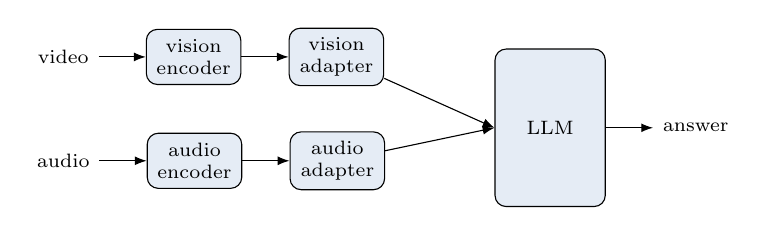
\begin{tikzpicture}[font=\scriptsize,>={Latex[length=1.5mm]},node distance=3.5mm and 6mm,
  enc/.style={draw,rounded corners,fill=frz!12,minimum width=12mm,minimum height=7mm,align=center},
  llm/.style={draw,rounded corners,fill=frz!12,minimum width=14mm,minimum height=20mm,align=center},
  io/.style={align=center}]
  \node[io] (vin) {video};
  \node[enc,right=of vin] (venc) {vision\\encoder};
  \node[enc,right=of venc] (vproj) {vision\\adapter};
  \node[io,below=9mm of vin] (ain) {audio};
  \node[enc,right=of ain] (aenc) {audio\\encoder};
  \node[enc,right=of aenc] (aproj) {audio\\adapter};
  \node[llm,right=14mm of vproj,yshift=-9mm] (llm) {LLM};
  \node[io,right=of llm] (ans) {answer};
  \draw[->] (vin)--(venc); \draw[->] (venc)--(vproj); \draw[->] (vproj)--(llm.west);
  \draw[->] (ain)--(aenc); \draw[->] (aenc)--(aproj); \draw[->] (aproj)--(llm.west);
  \draw[->] (llm.east)--(ans);
\end{tikzpicture}
\vspace{0.5em}
\begin{itemize}\small
\item Each modality is encoded into \textbf{tokens} (audio $\sim$25/s, video $\sim$100s--1000s per clip),
projected by a small \emph{adapter} into the LLM's embedding space, and concatenated with the question.
\item The LLM then answers over the \textbf{mixed token sequence} --- text, audio and vision compete
for its attention.
\item Examples: Qwen3-Omni (30B MoE), Qwen2.5-Omni (7B), VideoLLaMA2 --- our three test beds.
\end{itemize}
\end{frame}

% ============ 3. The failure ============
\begin{frame}{The failure we study: cross-modal hallucination}
\centering
\begin{tabular}{@{}c@{}}
\exrow{avh_a2v}{\textbf{audio $\to$ video}}{``Is the power tool visible?'' --- it is not.}{``Yes''}{``No''} \\[2.5mm]
\exrow{avh_v2a}{\textbf{video $\to$ audio}}{``Is the bird making sound?'' --- it is silent.}{``Yes''}{``No''}
\end{tabular}
\vfill
\small The model \textbf{over-trusts what it sees} and \textbf{under-uses what it hears}: it invents
sounds the image implies, and sees objects the audio suggests. One modality corrupts the other.
\end{frame}

% ============ 4. Research question ============
\begin{frame}{The research question}
\begin{center}\Large\itshape
Can we make a \textbf{frozen} AV-LLM ground its answers in what it hears\\[2pt]
--- by training something \textbf{tiny} bolted onto it?
\end{center}
\vfill
\begin{itemize}\small
\item \textbf{Frozen}: we never touch the 7--30B backbone --- cheap, safe, reversible.
\item \textbf{Tiny}: a $\sim$30M-parameter module per modality ($<$0.5\% of the model).
\item Constraint that shapes everything: the module must be \textbf{exactly invisible at initialization}
(so attaching it changes nothing until it learns something).
\end{itemize}
\end{frame}

% ============ 5. Benchmark I: AVHBench ============
\begin{frame}{Benchmark I --- AVHBench (the target)}
\begin{columns}[T]
\begin{column}{0.5\textwidth}
\footnotesize
\setlength{\tabcolsep}{4pt}
\begin{tabular}{@{}lrrr@{}}
\toprule
Judgment task & QnA & yes & no \\
\midrule
A$\to$V (audio$\to$video) & 1,136 & 568 & 568 \\
V$\to$A (video$\to$audio) & 2,290 & 1,145 & 1,145 \\
A--V Matching             & 1,876 & 938 & 938 \\
\midrule
\textbf{Total}            & \textbf{5,302} & 2,651 & 2,651 \\
\bottomrule
\end{tabular}
\par\vspace{0.4em}
{\scriptsize 2,136 everyday videos; yes/no \textbf{exactly balanced}, so a constant answer scores
50\% --- accuracy is honest.}
\end{column}
\begin{column}{0.5\textwidth}\scriptsize
\textbf{The three yes/no tasks}
\begin{itemize}
\item \textbf{A$\to$V}: ``is the queried object \emph{visible}?'' --- the \emph{heard} event tempts a
false yes.
\item \textbf{V$\to$A}: ``is the queried sound \emph{audible}?'' --- the \emph{seen} event tempts a
false yes. \textbf{Our audio-grounding probe.}
\item \textbf{A--V Matching}: ``do audio and video \emph{match}?'' --- needs real cross-modal
integration.
\end{itemize}
\end{column}
\end{columns}
\end{frame}

% ============ 6. Benchmark II: CMM ============
\begin{frame}{Benchmark II --- CMM (the capability guard)}
\centering
{\footnotesize \textbf{1,200 samples $\times$ 2 probes $=$ 2,400 questions}: one \emph{present} object
(gold ``yes''), one \emph{absent} (gold ``no'') per sample.}
\vspace{0.5em}
\[
\mathbf{PA}=\frac{\#\,\text{correct ``yes''}}{\#\,\text{ground-truth ``yes''}}
\qquad\qquad
\mathbf{HR}=\frac{\#\,\text{correct ``no''}}{\#\,\text{ground-truth ``no''}}
\]
\vspace{0.2em}
\begin{center}
\setbeamercolor{block body}{bg=red!6}
\begin{block}{Why you must watch BOTH numbers}
\centering\small A model that answers ``no'' to everything gets \textbf{HR $=$ 1.0} (never hallucinates!)
but \textbf{PA $=$ 0} (perceives nothing). Any hallucination fix must be checked against the trap of
just \emph{saying no more often}.
\end{block}
\end{center}
\vfill
{\footnotesize This trap is not hypothetical --- it is exactly what our first training run did.}
\end{frame}

% ============ 7. The adapter ============
\begin{frame}{Our module: a variational bottleneck on each modality stream}
\centering
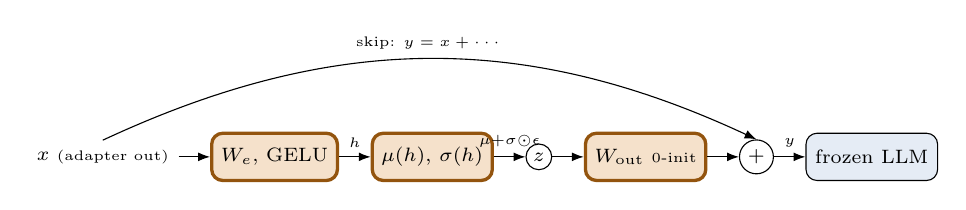
\begin{tikzpicture}[font=\scriptsize,>={Latex[length=1.5mm]},node distance=2mm and 4mm,
  trn/.style={draw,very thick,rounded corners,fill=trn!22,draw=trn!70!black,minimum height=6mm,align=center},
  frzs/.style={draw,rounded corners,fill=frz!12,minimum height=6mm,align=center},
  op/.style={draw,circle,inner sep=1.5pt},
  io/.style={align=center}]
  \node[io] (x) {$x$ {\tiny(adapter out)}};
  \node[trn,right=of x] (enc) {$W_e$, GELU};
  \node[trn,right=of enc] (ms) {$\mu(h),\,\sigma(h)$};
  \node[op,right=of ms] (z) {$z$};
  \node[trn,right=of z] (wout) {$W_{\text{out}}$ {\tiny 0-init}};
  \node[op,right=of wout] (add) {$+$};
  \node[frzs,right=of add] (llm) {frozen LLM};
  \draw[->] (x)--(enc); \draw[->] (enc)--node[above]{\tiny $h$}(ms);
  \draw[->] (ms)--node[above]{\tiny $\mu{+}\sigma{\odot}\epsilon$}(z);
  \draw[->] (z)--(wout); \draw[->] (wout)--(add);
  \draw[->] (add)--node[above]{\tiny $y$}(llm);
  \draw[->] (x.north) to[out=25,in=155] node[above,pos=0.5]{\tiny skip: $y=x+\cdots$} (add.north);
\end{tikzpicture}
\vspace{0.4em}
\[ z=\mu(x)+\sigma(x)\odot\epsilon \qquad y = x + W_{\text{out}}\,z \qquad W_{\text{out}}\stackrel{\text{init}}{=}0 \]
\begin{itemize}\small
\item \textbf{Zero-init} $\Rightarrow$ $y=x$ at the start: attaching it changes \emph{nothing} until trained.
\item A \texttt{bypass} switch gives the \textbf{exact frozen base for free} --- crucial for the training
objective (no second model in memory).
\item One per modality (audio, vision); together $<$0.5\% of the backbone's parameters.
\end{itemize}
\end{frame}

% ============ 8. The training trick ============
\begin{frame}{The training signal: manufacture an audio--vision conflict}
\centering
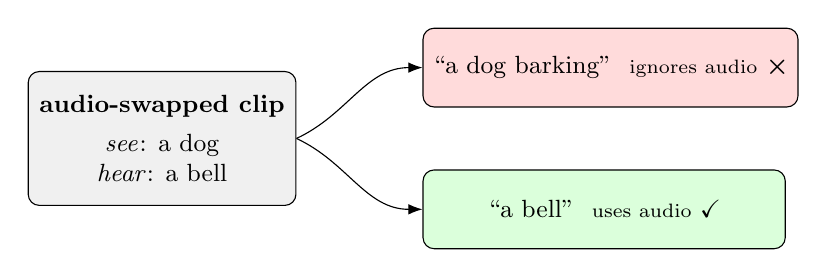
\begin{tikzpicture}[font=\small,>={Latex[length=1.8mm]},
  clip/.style={draw,rounded corners,fill=gray!12,align=center,minimum width=34mm,minimum height=17mm},
  good/.style={draw,rounded corners,fill=green!14,align=center,minimum width=46mm,minimum height=10mm},
  bad/.style={draw,rounded corners,fill=red!14,align=center,minimum width=46mm,minimum height=10mm}]
  \node[clip] (clip) {\textbf{audio-swapped clip}\\[1mm]\emph{see}: a dog\\\emph{hear}: a bell};
  \node[bad,right=16mm of clip,yshift=9mm] (bad) {``a dog barking'' \ {\scriptsize ignores audio} $\boldsymbol{\times}$};
  \node[good,right=16mm of clip,yshift=-9mm] (good) {``a bell'' \ {\scriptsize uses audio} $\boldsymbol{\checkmark}$};
  \draw[->] (clip.east) to[out=25,in=180] (bad.west);
  \draw[->] (clip.east) to[out=-25,in=180] (good.west);
\end{tikzpicture}
\vspace{0.4em}
\par
\exrow{as_flute}{\emph{see} flute, \textbf{hear (overlaid) train horn}}{``Which event do you hear?''}{``flute''}{``train horn''}
\vfill
\small Swap a clip's audio track (one \texttt{ffmpeg} call) $\Rightarrow$ seen $\neq$ heard. Preferring
the \textbf{heard} answer on the \emph{same} clip is only possible by \textbf{using the audio}.
\end{frame}

% ============ 9. What broke ============
\begin{frame}{First attempt: na\"ive preference optimization collapses}
\begin{itemize}
\item Train with standard DPO on the swap pairs $\Rightarrow$ perception accuracy
\textbf{0.95 $\to$ 0.1}; the model converges to answering ``no'' to \emph{everything}.
\item Mechanism (\emph{likelihood displacement}): the DPO margin can grow while \textbf{both}
answers' probabilities \emph{fall} --- the loss is satisfied by destroying the model.
\item And remember the CMM trap: all-``no'' looks \textbf{perfect} on hallucination metrics.
\end{itemize}
\vfill
\begin{center}
\setbeamercolor{block body}{bg=red!8}
\begin{block}{}
\centering\small First lesson of this project: \textbf{a hallucination metric alone cannot be your
training target.}
\end{block}
\end{center}
\end{frame}

% ============ 10. The fix ============
\begin{frame}{The fix: one engine, two safety rails}
\vspace{-0.3em}
\begin{align*}
\mathcal L =\ & \underbrace{-\log\sigma(\beta[(c_p{-}c_r){-}(r_p{-}r_r)])}_{\text{\textbf{engine}: prefer the heard answer}}
 \;+\; \lambda_a\,\underbrace{\big({-}\log\sigma(\beta(c_p{-}c_r){-}\delta)\big)}_{\textcolor{trn}{\textbf{rail 1}: chosen $\ge$ base $\Rightarrow$ PA}} \\[2pt]
 &+\; \lambda_{kl}\,\underbrace{\mathrm{KL}\!\big(p_{\text{base}}\,\|\,p_\theta\big)}_{\textcolor{trn}{\textbf{rail 2}: normal inputs unchanged $\Rightarrow$ HR}}
 \;+\; \beta_{kl}\,\mathrm{KL}_{\text{VIB}}
\end{align*}
\vspace{-0.3em}
\begin{itemize}\small
\item $c,r$ $=$ log-probs of the chosen (heard) / rejected (seen) answer; $p$ $=$ adapter on,
$r$-subscript $=$ adapter \emph{bypassed} $=$ the frozen base.
\item \textbf{Rail 1} forbids the collapse route: the chosen answer may never sink below its base
probability. \textbf{Rail 2} pins behavior on ordinary (non-swap) inputs.
\item Result: answering ``no'' to everything now \emph{fires both rails} --- the only way to lower the
engine's loss is to actually use the audio.
\end{itemize}
\end{frame}

% ============ 11. Results ============
\begin{frame}{Results (Qwen3-Omni, full benchmark, n$=$5302)}
\centering
\renewcommand{\arraystretch}{1.2}
\footnotesize
\begin{tabular}{l cccc cc}
\toprule
& \multicolumn{4}{c}{AVHBench} & \multicolumn{2}{c}{CMM} \\
\cmidrule(lr){2-5}\cmidrule(lr){6-7}
 & $A\!\to\!V$ & $V\!\to\!A$ & AV-m & overall & PA & HR \\
\midrule
frozen base              & \textbf{0.838} & 0.812 & 0.653 & 0.761 & \textbf{0.900} & 0.733 \\
+ swap-DPO adapter       & 0.837 & \textbf{0.838} & 0.766 & 0.812 & 0.890 & 0.743 \\
+ FiLM adapter (prompt-aware) & 0.822 & 0.827 & \textbf{0.808} & \textbf{0.819} & 0.894 & \textbf{0.746} \\
\midrule
+ LoRA (same recipe)     & \XXX & \XXX & \XXX & \XXX & \XXX & \XXX \\
+ MoD-DPO (baseline)     & \XXX & \XXX & \XXX & \XXX & \XXX & \XXX \\
+ MoD-DPO++ (baseline)   & \XXX & \XXX & \XXX & \XXX & \XXX & \XXX \\
MAD decoding (training-free) & \XXX & \XXX & \XXX & \XXX & \XXX & \XXX \\
+ cross-attention fusion & \XXX & \XXX & \XXX & \XXX & \XXX & \XXX \\
\bottomrule
\end{tabular}
\vfill
{\small Both adapters give a real gain with \textbf{capability preserved} (HR does not drop) ---
the two anchors doing their job. \XXX{} rows: baselines training/evaluating \emph{right now}.}
\end{frame}

% ============ 12. Are the gains real? ============
\begin{frame}{Are the gains real? Paired statistics in three lines}
{\small Both models answer the \textbf{same} items, so only \textbf{disagreements} carry information:
out of $N$ items, $b$ $=$ only-base-right, $c$ $=$ only-adapter-right.}
\[
\Delta=\frac{c-b}{N}\qquad\quad
\text{95\% CI: }\Delta\pm 1.96\cdot\frac{\sqrt{(b+c)-(c-b)^2/N}}{N}
\qquad\quad
\text{McNemar: is } b/c \text{ a fair coin?}
\]
\vspace{0.2em}
\centering
\footnotesize
\begin{tabular}{l c c c}
\toprule
comparison & $b$ / $c$ & $\Delta$ [95\% CI] & verdict \\
\midrule
base $\to$ swap-DPO & 152 / 411 & $+5.2$ [{+}4.3, {+}6.1] & real ($p<10^{-4}$) \\
base $\to$ FiLM     & 253 / 532 & $+5.6$ [{+}4.5, {+}6.7] & real ($p<10^{-4}$) \\
DPO $\to$ FiLM      & 204 / 224 & $+0.4$ [{-}0.4, {+}1.2] & tie overall --- FiLM wins AV-Matching ($+3.7$, $p<10^{-4}$) \\
\bottomrule
\end{tabular}
\vfill
{\small 411 fixed vs 152 broken cannot be a coin flip --- that is the entire test.}
\end{frame}

% ============ 13. FiLM ============
\begin{frame}{FiLM: let the \emph{question} steer the adapter}
\centering
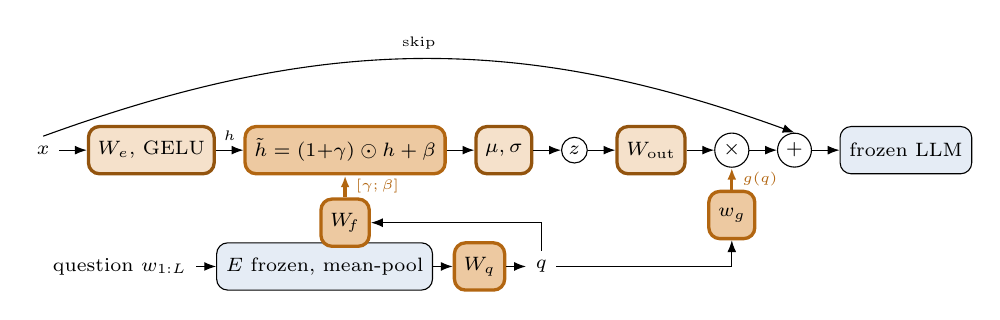
\begin{tikzpicture}[font=\scriptsize,>={Latex[length=1.5mm]},node distance=2mm and 3.5mm,
  trn/.style={draw,very thick,rounded corners,fill=trn!22,draw=trn!70!black,minimum height=6mm,align=center},
  new/.style={draw,very thick,rounded corners,fill=trn!40,draw=trn!85!black,minimum height=6mm,align=center},
  frzs/.style={draw,rounded corners,fill=frz!12,minimum height=6mm,align=center},
  op/.style={draw,circle,inner sep=1.5pt},
  io/.style={align=center}]
  \node[io] (x) {$x$};
  \node[trn,right=of x] (enc) {$W_e$, GELU};
  \node[new,right=of enc] (film) {$\tilde h=(1{+}\gamma)\odot h+\beta$};
  \node[trn,right=of film] (ms) {$\mu,\sigma$};
  \node[op,right=of ms] (z) {$z$};
  \node[trn,right=of z] (wout) {$W_{\text{out}}$};
  \node[op,right=of wout] (mult) {$\times$};
  \node[op,right=of mult] (add) {$+$};
  \node[frzs,right=of add] (llm) {frozen LLM};
  \draw[->] (x)--(enc); \draw[->] (enc)--node[above]{\tiny $h$}(film);
  \draw[->] (film)--(ms); \draw[->] (ms)--(z);
  \draw[->] (z)--(wout); \draw[->] (wout)--(mult); \draw[->] (mult)--(add);
  \draw[->] (add)--(llm);
  \draw[->] (x.north) to[out=20,in=160] node[above,pos=0.5]{\tiny skip} (add.north);
  \node[io,below=13mm of x,anchor=west] (w) {question $w_{1:L}$};
  \node[frzs,right=2.5mm of w] (embed) {$E$ frozen, mean-pool};
  \node[new,right=2.5mm of embed] (wq) {$W_q$};
  \node[io,right=2.5mm of wq] (qv) {$q$};
  \node[new] (wf) at ([yshift=-6mm]film.south) {$W_{\!f}$};
  \node[new] (wg) at ([yshift=-6mm]mult.south) {$w_g$};
  \draw[->] (w)--(embed); \draw[->] (embed)--(wq); \draw[->] (wq)--(qv);
  \draw[->] (qv.north) |- (wf.east);
  \draw[->] (qv.east) -| (wg.south);
  \draw[->,trn!85!black,very thick] (wf.north)--node[right]{\tiny $[\gamma;\beta]$}(film.south);
  \draw[->,trn!85!black,very thick] (wg.north)--node[right]{\tiny $g(q)$}(mult.south);
\end{tikzpicture}
\vspace{0.4em}
\par
{\small The question becomes a vector $q$; it picks a per-feature \textbf{scale} $\gamma$ and
\textbf{shift} $\beta$ on the bottleneck (that is all ``FiLM'' is), plus one \textbf{volume knob}
$g(q)$ on the edit. Same zero-init trick $\Rightarrow$ identity at start.}
\end{frame}

% ============ 14. Why FiLM must read the question ============
\begin{frame}{Why the question \emph{must} be used (a 3-row proof)}
{\small One swapped clip: \emph{see} a dog, \emph{hear} a bell. Ask ``what do you HEAR?'' (answer: bell)
and ``what do you SEE?'' (answer: dog). \textbf{Same pixels, same waveform --- only the question differs.}
Loss per question $=-\log\sigma(m)$: $m{=}{+}2\!\to\!0.13$, $m{=}0\!\to\!0.69$, $m{=}{-}2\!\to\!2.13$.}
\vspace{0.4em}
\centering
\renewcommand{\arraystretch}{1.15}
\footnotesize
\begin{tabular}{l l cc c}
\toprule
adapter & answers (HEAR / SEE) & HEAR loss & SEE loss & total \\
\midrule
can't read $q$, commits to ``bell'' & ``bell'' / ``bell'' & $0.13$ & $2.13$ & $2.26$ \\
can't read $q$, hedges 50/50        & --- & $0.69$ & $0.69$ & $\mathbf{1.39}$ (floor) \\
\textbf{reads $q$}                  & ``bell'' / ``dog''  & $0.13$ & $0.13$ & $\mathbf{0.26\to 0}$ \\
\bottomrule
\end{tabular}
\vspace{0.5em}
\par
{\small Question-blind adapters are stuck $\ge 2\log 2\approx 1.39$ per pair; question-aware ones reach
$0$ $\Rightarrow$ training \textbf{forces} the adapter to use the question. No regularizer needed ---
the \emph{data construction} does it.}
\end{frame}

% ============ 15. Mechanism: attention ============
\begin{frame}{Does the adapter make the model \emph{attend} to the audio--visual input?}
\begin{columns}[T]
\begin{column}{0.58\textwidth}
\centering
\figslot{attn_av.png}{\linewidth}\\[2pt]
{\scriptsize Share of the answer position's attention landing on audio/visual tokens, per clip
(box $=$ median/IQR). Compare \textbf{within} a model only.}
\end{column}
\begin{column}{0.42\textwidth}\small
\begin{itemize}\footnotesize
\item base $\to$ swap-DPO: $\approx$ flat (5.4\% $\to$ 5.7\%) --- it grounds by \emph{re-encoding} the
tokens, not by looking at them more.
\item base $\to$ \textbf{FiLM}: \textbf{5.4\% $\to$ 7.4\%} ($+38\%$) --- the only variant that
\emph{attends more} to the evidence.
\end{itemize}
\vspace{0.4em}
{\footnotesize Same benchmark gain, \textbf{two different mechanisms} --- and only one is the mechanism
we actually claimed. Finding this required measuring, not assuming.}
\end{column}
\end{columns}
\end{frame}

% ============ 16. Mechanism: the listening test ============
\begin{frame}{A second probe: does the answer \emph{depend} on the audio?}
\begin{columns}[T]
\begin{column}{0.56\textwidth}
\centering
\figslot{ll_shift.png}{\linewidth}\\[2pt]
{\scriptsize \emph{Illustration of the probe.} KDE of the gold answer's log-likelihood with
\textcolor{teal}{true} vs \textcolor{magenta}{swapped} audio; the \textbf{shift} of the means is an
audio-reliance meter.}
\end{column}
\begin{column}{0.44\textwidth}\small
\begin{itemize}\footnotesize
\item Swap the audio, re-score the \emph{same} answer: a model that ignores audio shifts $\approx 0$.
\item Measured shifts: base \XXX{}\quad$\cdot$\quad $+$DPO \XXX{}\quad$\cdot$\quad $+$FiLM \XXX{}
(runs in flight).
\end{itemize}
\vspace{0.4em}
{\footnotesize Two independent probes (attention $+$ likelihood) triangulate the mechanism ---
one alone can mislead.}
\end{column}
\end{columns}
\end{frame}

% ============ 17. Baselines in flight ============
\begin{frame}{What we are comparing against (running right now)}
\centering
\renewcommand{\arraystretch}{1.3}
\footnotesize
\begin{tabular}{l l l}
\toprule
method & type & one-line idea \\
\midrule
LoRA (same attach points) & trained control & is it just ``any adapter''? \\
MoD-DPO / ++ {\tiny(arXiv:2603.03192)} & training objective & DPO $+$ invariance/sensitivity to corrupted modalities \\
MAD {\tiny(arXiv:2601.21181)} & \textbf{training-free decoding} & ask the model which modality matters; contrast 4 input configs \\
cross-attention fusion & trained arm & audio$\leftrightarrow$vision attention before the LLM \\
\bottomrule
\end{tabular}
\vfill
\begin{itemize}\small
\item All four run through \textbf{the same harness} (same prompts, same items, paired statistics) ---
otherwise the comparison is meaningless.
\item Results: \XXX{} (jobs submitted this morning; the table on slide 11 fills itself in).
\end{itemize}
\end{frame}

% ============ 18. What did not work ============
\begin{frame}{What did \emph{not} work --- and what each failure taught}
\centering
\renewcommand{\arraystretch}{1.3}
\scriptsize
\begin{tabular}{l l l}
\toprule
tried & failure & lesson \\
\midrule
na\"ive swap-DPO & collapse to constant ``no'' (PA $0.95\!\to\!0.1$) & metrics can be gamed $\to$ two anchors \\
GRPO on easy yes/no & zero advantage on 2/3 of steps: no gradient & unanimous rewards teach nothing $\to$ harder items \\
FiLM's hard gate $g(q)$ & never closed (stayed at init) & the model preferred \emph{modulation} over routing \\
``vision rewrites 59\%'' story & overturned by auditing the weights & \textbf{measure, don't assume} \\
\bottomrule
\end{tabular}
\vfill
{\small Half of these failures became the paper's actual \emph{content}. Negative results are data.}
\end{frame}

% ============ 19. Methodology ============
\begin{frame}{The part that saved us: evaluation hygiene}
\begin{itemize}\small
\item \textbf{The harness is a lever.} Changing only the answer-format suffix moved a model's score by
$+11$ points on one axis (V$\to$A $69.0\to80.3$) --- \emph{same weights}. Pin fps, prompts, suffixes.
\item \textbf{Never select on the test set}: pick checkpoints on a validation half, report on the
disjoint rest. Our first ``best'' checkpoint didn't survive this.
\item \textbf{Paired statistics or it didn't happen}: same items, McNemar $+$ bootstrap CI.
\item \textbf{Watch the trap metric} (yes-rate / PA) --- the failure mode that looks like success.
\item \textbf{Leakage check}: training clips $\cap$ benchmark clips $=\varnothing$, scripted.
\end{itemize}
\vfill
\begin{center}
\setbeamercolor{block body}{bg=blue!6}
\begin{block}{}
\centering\small If you remember one slide from this talk, make it this one.
\end{block}
\end{center}
\end{frame}

% ============ 20. Open problems ============
\begin{frame}{Open problems (things you could work on)}
\begin{itemize}\small
\item \textbf{Causal mechanism}: bypass one modality's adapter at a time --- which one carries the gain?
\item \textbf{Composition}: training-free decoding (MAD/AVCD) \emph{on top of} the trained adapter.
\item \textbf{Make the bottleneck bite}: the IB rate barely binds at our $\beta_{kl}$ --- is there a
regime where compression itself helps?
\item \textbf{Backbone prerequisite}: the gain tracks how much the frozen model already uses audio
(null on VideoLLaMA2) --- can an adapter \emph{create} audio use where there is none?
\item \textbf{Scale}: 600 swapped clips saturate our recipe --- what unlocks the next tier, data or
objective?
\end{itemize}
\vfill
{\footnotesize Everything is reproducible from the repo: one script per table, one command per figure.}
\end{frame}

% ============ 21. Summary ============
\begin{frame}{Summary}
\begin{itemize}
\item \textbf{Problem}: frozen AV-LLMs over-trust vision; audio evidence loses.
\item \textbf{Method}: a tiny zero-init adapter $+$ audio-swap preference training $+$ two anchors
against collapse.
\item \textbf{Result}: $+5$--$6$ AVHBench points, statistically solid, capability intact ---
and the prompt-aware (FiLM) variant does it by a \emph{faithful} mechanism.
\item \textbf{Honesty}: the harness, the selection protocol and the paired statistics mattered as much
as the method.
\item \textbf{In flight}: LoRA / MoD-DPO / MAD / cross-attention comparisons --- \XXX{} until the jobs
finish.
\end{itemize}
\vfill
\begin{center}
{\large Questions --- or come run one of the \XXX{} cells yourself.}
\end{center}
\end{frame}

\end{document}
